\documentclass[11pt]{report}
\usepackage[utf8]{inputenc}
\usepackage[a4paper, margin=1in]{geometry}
\usepackage{graphicx, color}
\usepackage{booktabs}
\usepackage[toc,page]{appendix}
\usepackage{pdfpages}
\usepackage{multicol}
\usepackage{changepage}
\usepackage{float}
\usepackage{multirow}
\usepackage{amsmath}
\usepackage[encoding,filenameencoding=utf8]{grffile}
\usepackage{subcaption}
\usepackage{csquotes}
\usepackage{hyperref, bookmark}

\setlength{\columnseprule}{0.5pt}
\def\columnseprulecolor{\color{black}}


% Package de algoritmos
\usepackage[portuguese,ruled,lined]{algorithm2e}

% Portuguese Encoding 
\usepackage[portuguese]{babel}
\usepackage[T1]{fontenc}

% import Java
\usepackage{listings} 

% Header
\usepackage{fancyhdr}
\pagestyle{fancy}
	\fancyhf{}
		\lhead{LEIC - ISEL}
    \rhead{Segurança Informática}

% Footer
\renewcommand{\headrulewidth}{1pt}
\renewcommand{\footrulewidth}{1pt}
\fancyfoot[CE,CO]{\thepage}


%%%%%%%%%%%%%%%%%%%%%%%%%%%%%%%%%%%%%%%%% CHANGES %%%%%%%%%%%%%%%%%%%%%%%%%%%%%%%%%


% Redefine the plain page style
\fancypagestyle{plain}{
\pagestyle{fancy}
  \fancyhf{}
	\lhead{LEIC - ISEL}
	\rhead{Segurança Informática}
	\renewcommand{\headrulewidth}{1pt}
	\renewcommand{\footrulewidth}{1pt}
\fancyfoot[CE,CO]{\thepage}
}

%%%%%%%%%%%%%%%%%%%%%%%%%%%%%%%%%%%%%%%%% CHANGES %%%%%%%%%%%%%%%%%%%%%%%%%%%%%%%%%

% Titulo e informação de capa
\title{Primeira Serie de exercícios}
\date{Outubro 2019}

% Define Chapter heading
\makeatletter
\def\@makechapterhead#1{%
  \vspace*{20\p@}%                                 % Insert 50pt (vertical) space
  {\parindent \z@ \raggedright \normalfont         % No paragraph indent, ragged right
%    \interlinepenalty\@M                           % Penalty
    \huge \bfseries #1\par\nobreak                 % Huge, bold chapter title
    \vskip 10\p@                                   % Insert 40pt (vertical) space
  }}
  
  %%%%%%%%%%%%%%%%%%%%%%%%%%%%%%%%%%%%%%%%% CHANGES %%%%%%%%%%%%%%%%%%%%%%%%%%%%%%%%%

\makeatother

%Custom commands

\renewcommand\appendixpagename{Anexos}
\renewcommand\appendixname{Anexo}
\renewcommand\appendixtocname{Anexos}

\newenvironment{subs}
  {\adjustwidth{2.5em}{0pt}}
  {\endadjustwidth}


% Retira a indentação ao início dos parágrafos 
\setlength{\parindent}{0em}
\newcommand{\blank}[1]{\hspace*{#1}\linebreak[0]}

% Section and Subsection spacing:
\usepackage{titlesec}
\usepackage{lipsum}



%%%%%%%%%%%%%%%%%%%%%%%%%%%%%%%%%%	DOCUMENT BEGINS	%%%%%%%%%%%%%%%%%%%%%%%%%%%%%%%%%%%%%

\begin{document}

%%%%%%%%%%%%%%%%%%%%%%%%%%%%%%%%%%%%%%%%%%%%%%%%%%%%%%%%%%%%%%%%%%%%%%%%%%%%%%%%%%%%%%%%%
%										COVER											%
%%%%%%%%%%%%%%%%%%%%%%%%%%%%%%%%%%%%%%%%%%%%%%%%%%%%%%%%%%%%%%%%%%%%%%%%%%%%%%%%%%%%%%%%%

\begin{titlepage} 

\newcommand{\HRule}{\rule{\linewidth}{0.5mm}} % Defines a new command for the horizontal lines, change thickness here

%----------------------------------------------------------------------------------------
%	LOGO SECTION
%----------------------------------------------------------------------------------------


\includegraphics[width=130pt, keepaspectratio=true]{img/logo_isel}\\[1cm] % Include a department/university logo - this will require the graphicx package
\center % Center everything on the page
 
%----------------------------------------------------------------------------------------
%	HEADING SECTIONS
%----------------------------------------------------------------------------------------

\textsc{\LARGE INSTITUTO SUPERIOR DE ENGENHARIA DE LISBOA}\\[1.5cm] % Name of your university/college
\vskip 40pt
\textsc{\Large SEGURANÇA INFORMÁTICA}\\[0.5cm] % Major heading such as course name
\textsc{\large LICENCIATURA ENGENHARIA INFORMÁTICA E COMPUTADORES}\\[0.5cm] % Minor heading such as course title
\vskip 40pt

%----------------------------------------------------------------------------------------
%	TITLE SECTION
%----------------------------------------------------------------------------------------

\HRule \\[0.4cm]
{ \LARGE \bfseries SÉRIE DE EXERCÍCIOS }\\[0.4cm]
{ \huge \bfseries Fase 3}\\[0.4cm] % Title of your document
\HRule \\[1.5cm]
 
%----------------------------------------------------------------------------------------
%	AUTHOR SECTION
%----------------------------------------------------------------------------------------
\vskip 70pt
\begin{minipage}{0.4\textwidth}
\begin{flushleft} \large
\emph{Autores:}\\
43552 - Samuel \textsc{Costa}\\
43320 - André \textsc{Mendes}
\end{flushleft}
\end{minipage}
~
\begin{minipage}{0.4\textwidth}
\begin{flushright} \large
\emph{Docente:} \\
José \textsc{Simão}\\
\end{flushright}
\end{minipage}\\[3cm]

%----------------------------------------------------------------------------------------
%	DATE SECTION
%----------------------------------------------------------------------------------------

{\large 05 de Dezembro de 2019}\\[3cm] % Date, change the \today to a set date if you want to be precise

%----------------------------------------------------------------------------------------

\vfill % Fill the rest of the page with whitespace

\end{titlepage}


\renewcommand\thesection{\arabic{section}}

\pdfbookmark{\contentsname}{toc}
\tableofcontents


\newpage


\section*{Introdução}
O trabalho realizado para este fase pretende que os temas desenvolvidos durante as aulas sejam postos em prática. Para esta fase os exercícios focaram essencialmente a segunda parte da matéria.\\

\begin{itemize}
  \item Modelos de Controlo de Acesso
  \item Vulnerabilidades em aplicações nativas, base de dados e web
\end{itemize}

Neste trabalho prático pretendemos responder aos vários exercícios propostos e implementar uma demonstração dos pontos referidos.

\newpage


\section{Exercício 1}
	Ambos são elementos do sistema de controlo de acessos (autorização). O modelo define as regras gerais seguidas no âmbito da autorização, enquanto as políticas são a concretização do modelo. No contexto do Sistema Operativo, identificamos a matriz de acesso como um modelo de controlo de acessos, tendo como sua concretização (política) a lista de controlo de acessos.

\section{Exercício 2}
	\subsection*{2.1}
	Uma vez que o modelo RBAC1 comporta a hierarquia de papeis, é possível a existência de uma sessão com um user u com o role activo r, sem que (u,r) esteja na relação UA, se o utilizador tiver o role r1 e r <= r1.
	
	\subsection*{2.2}
	O princípio de privilégios mínimos indica que por omissão se deve restringir os privilégios de acesso.
	Quando aplicado aos utilizadores, quer dizer que todos os utilizadores devem sempre utilizar o sistema com o mínimo de privilégios possível.
	Como princípio geral, o desenho do sistema deve conceder as permissões mínimas aos roles para executarem as ações necessárias, proibindo por omissão, em vez de proibir como excepção.

\section{Exercício 3}
	Em CVE-2019-9766 trata-se de uma vulnerabilidade buffer-overflow baseada no stack. Esta vulnerabilidade é causada pela coincidência no stack de dados do programa (variáveis locais à função) e dados de controlo de fluxo (endereço de retorno para função chamadora e endereço do início da frame anterior). Se a escrita numa variável local exceder os limites dos dados do programa e esmagar os dados de controlo de fluxo, quando a função retornar pode ser executado código arbitrário. Neste caso, é a operação de conversão de um ficheiro que pode ser explorada, tirando partido da dimensão da zona do stack reservada a dados locais da função.

\section{Exercício 4}
	Tanto a vulnerabilidade buffer overflow como cross-site scripting dizem respeito à execução de código arbitrário.

\section{Exercício 5}
Se o atacante conseguisse explorar a vulnerabilidade CSRF da rota /googlecallback, fazendo a vítima efectuar um pedido GET para essa rota com um state válido e o seu code, a aplicação tentaria trocar o code pelo access token do atacante, no que seria bem sucedida. Se a vítima prosseguisse o fluxo da aplicação, estaria a guardar os seus issues em tasks da conta do atacante.

\newpage

\section{Exercício 6}
	\subsection*{6.1}
	Foi iniciada uma instância com o id 472900268124152302695985496522790539409. A aplicação está disponível em https://google-gruyere.appspot.com/472900268124152302695985496522790539409/.
	Foi criada uma conta na app Gruyere com o utilizador LI51N-SI1920iG01 e a password gruyerepass.
	\subsection*{6.2}
	 \textbf{Upload XSS} - Foi elaborado o documento html upload\_xss2.html que contem um elemento script que executa a função alert com as cookies do utilizador. Depois de carregar o ficheiro para o servidor, acedeu-se ao url fornecido. Em resultado foi realizado pelo browser um pedido GET para uma rota dentro do mesmo domínio, o que implicou que o browser envia as cookies que possui para esse domínio, fazendo com que a informação presente nas cookies do utilizador fosse acessível ao documento carregado.
	 \newline
	 
	 \textbf{Reflected XSS} - Foi iniciada uma instância do browser com a flag --disable-xss-auditor. Foi elaborado o seguinte url:\newline https://google-gruyere.appspot.com/472900268124152302695985496522790539409/<script>\newline
	 alert(document.cookie);</script>\newline, que injecta no documento um elemento script que executa código arbitrário, tirando partido do facto de a aplicação encaminhar directamente os dados de entrada na mensagem que exibe ao utilizador.
	 \newline
	 
	 \textbf{Stored XSS} - A vulnerabilidade foi explorada criando um snippet com o seguinte conteúdo: <a onmouseover="alert(document.cookie)" href="\#">exploit!</a>, que regista um evento quando o utilizador passa o rato por cima do snippet, mostrando em janela de diálogo os cookies do utilizador.
	
	\subsection*{6.3}
	Como já vimos, a app Gruyere é vulnerável a ataques do tipo XSS (stored, upload e reflected). Para receber as cookies de uma vítima na sua app, o atacante necessita de confeccionar um script que, sem o conhecimento da vítima, faça um pedido GET para a sua aplicação com as cookies na query string.
	Como as cookies só estão disponíveis em documentos da mesma origem (SOP), o atacante precisa de injectar esse script numa página do domínio da aplicação Gruyere, o que já vimos que é possível.\newline
	O ataque foi executado, tendo sido verificada a existência de um documento na BD na rota siserie3-result da app do atacante.
	

	
\section{Exercício 7}
	\subsection*{7.1}
Autenticou-se o utilizador Alice na aplicação Elgg. Efetuou-se um pedido GET para a rota /profile/:user com user=alice. Constatou-se que nesse pedido foram enviados os headers referer e cookie com uma cookie com o nome Elgg.
De seguida, foi efectuado um pedido POST para a rota /action/friends/add. Além de ser enviado o header cookie com a mesma cookie do pedido GET, foram enviados na query string os seguintes parâmetros:
\begin{itemize}
	\item \_\_elgg\_token
	\item \_\_elgg\_ts
	\item friend	
\end{itemize}
O parâmetro friend é único por utilizador e não é alterado. Os parâmetros \_\_elgg\_token e \_\_elgg\_ts (timestamp) são gerados por cada pedido do formulário de edição do perfil.

	\subsection*{7.2}
	Foi configurado o adaptador de rede para funcionar no modo bridge. A figura 1 apresenta o ping feito com sucesso à VM-elgg e à VM-attacker.
	
	Configurou-se a aplicação do atacante em VM-attacker. Colocou-se o conteúdo do ficheiro anexo attacker.html em index.html. A partir deste momento, a aplicação que responde por 192.168.1.122 envia o ficheiro malicioso.
	
	Copiou-se a aplicação Elgg para a pasta /var/www/home da VM-elgg.
	
	Editou-se o documento hosts no host para que os endereços da app elgg e da app do atacante passem a ser resolvidos localmente. Adicionaram-se as seguintes duas linhas ao ficheiro:
	\begin{itemize}
		\item 192.168.1.122 www.csrflabattacker.com
		\item 192.168.1.123 www.csrflabelgg.com
	\end{itemize}
	Acedeu-se a partir da máquina host à aplicação Elgg para realizar login como o utilizador Alice. Abriu-se uma outra janela do browser para se aceder à aplicação atacante. A figura 2 mostra este passo do ataque. Em seguida, acedeu-se ao relatório de actividade da aplicação Elgg, de onde consta o efeito do ataque (Figura 3).
	
	
\begin{figure}[!htb]
	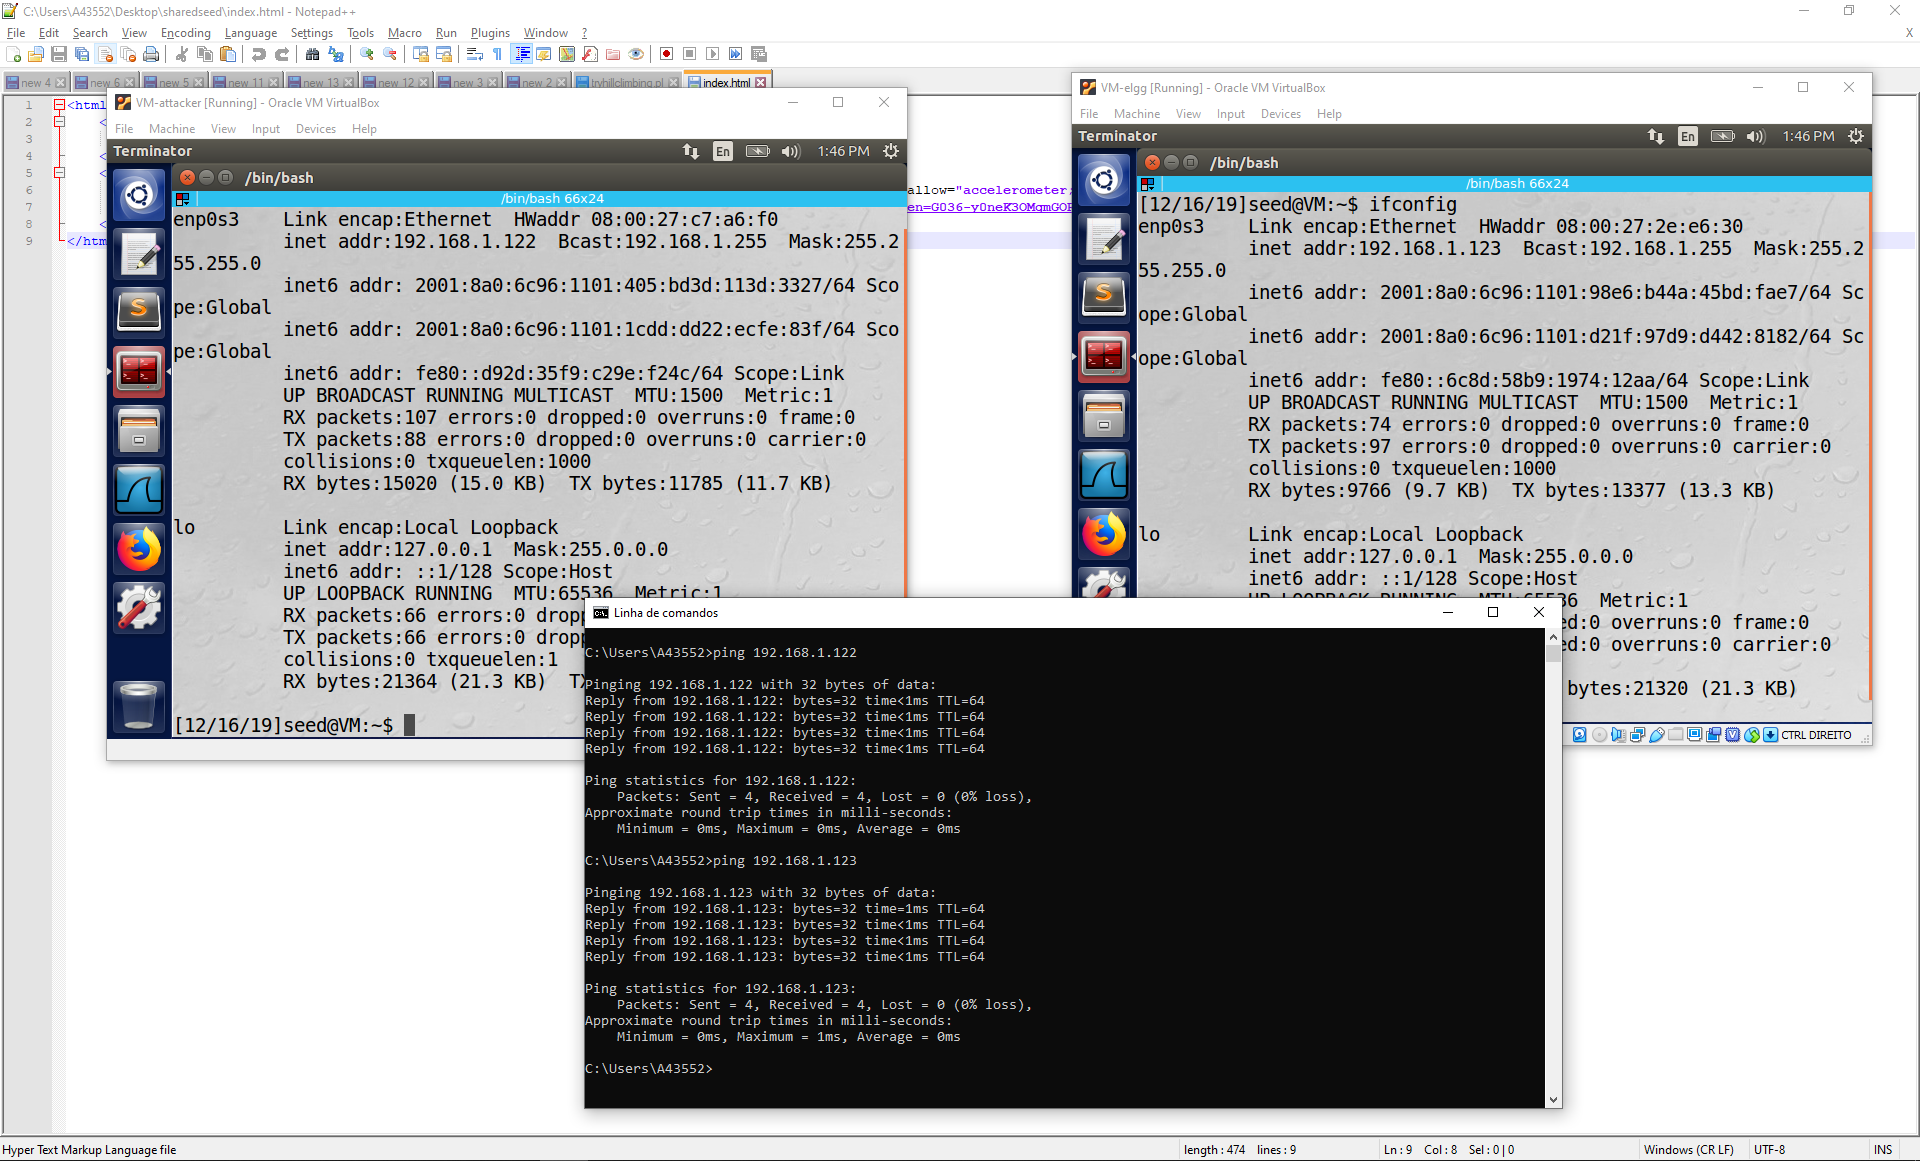
\includegraphics[width=\linewidth]{img/ping}
	\caption{Endereços IP das VM's e estabelecimento do ping desde a máquina host}
	\label{fig:ping}
\end{figure}
\begin{figure}[!htb]
	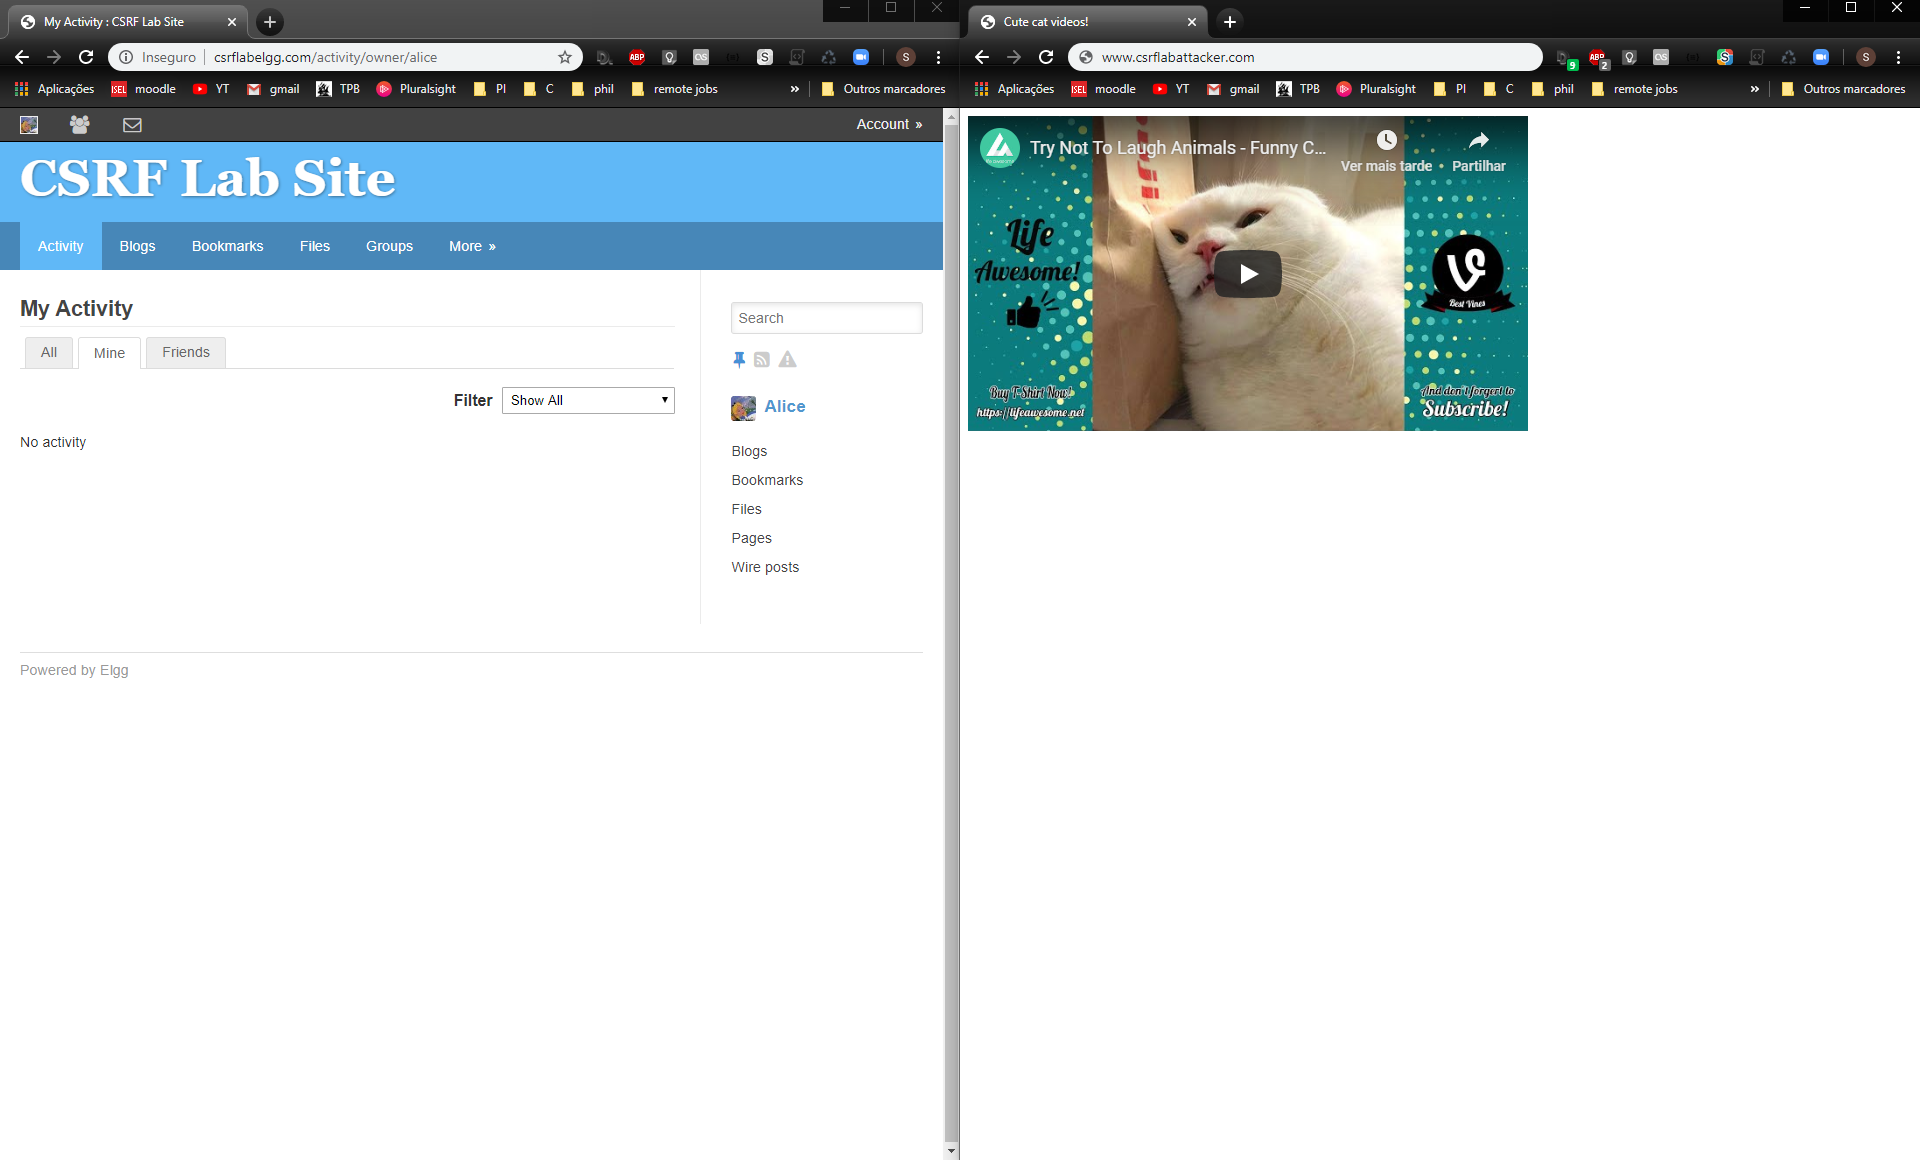
\includegraphics[width=\linewidth]{img/access}
	\caption{Vítima visita a aplicação atacante}
	\label{fig:access}
\end{figure}
\begin{figure}[!htb]
	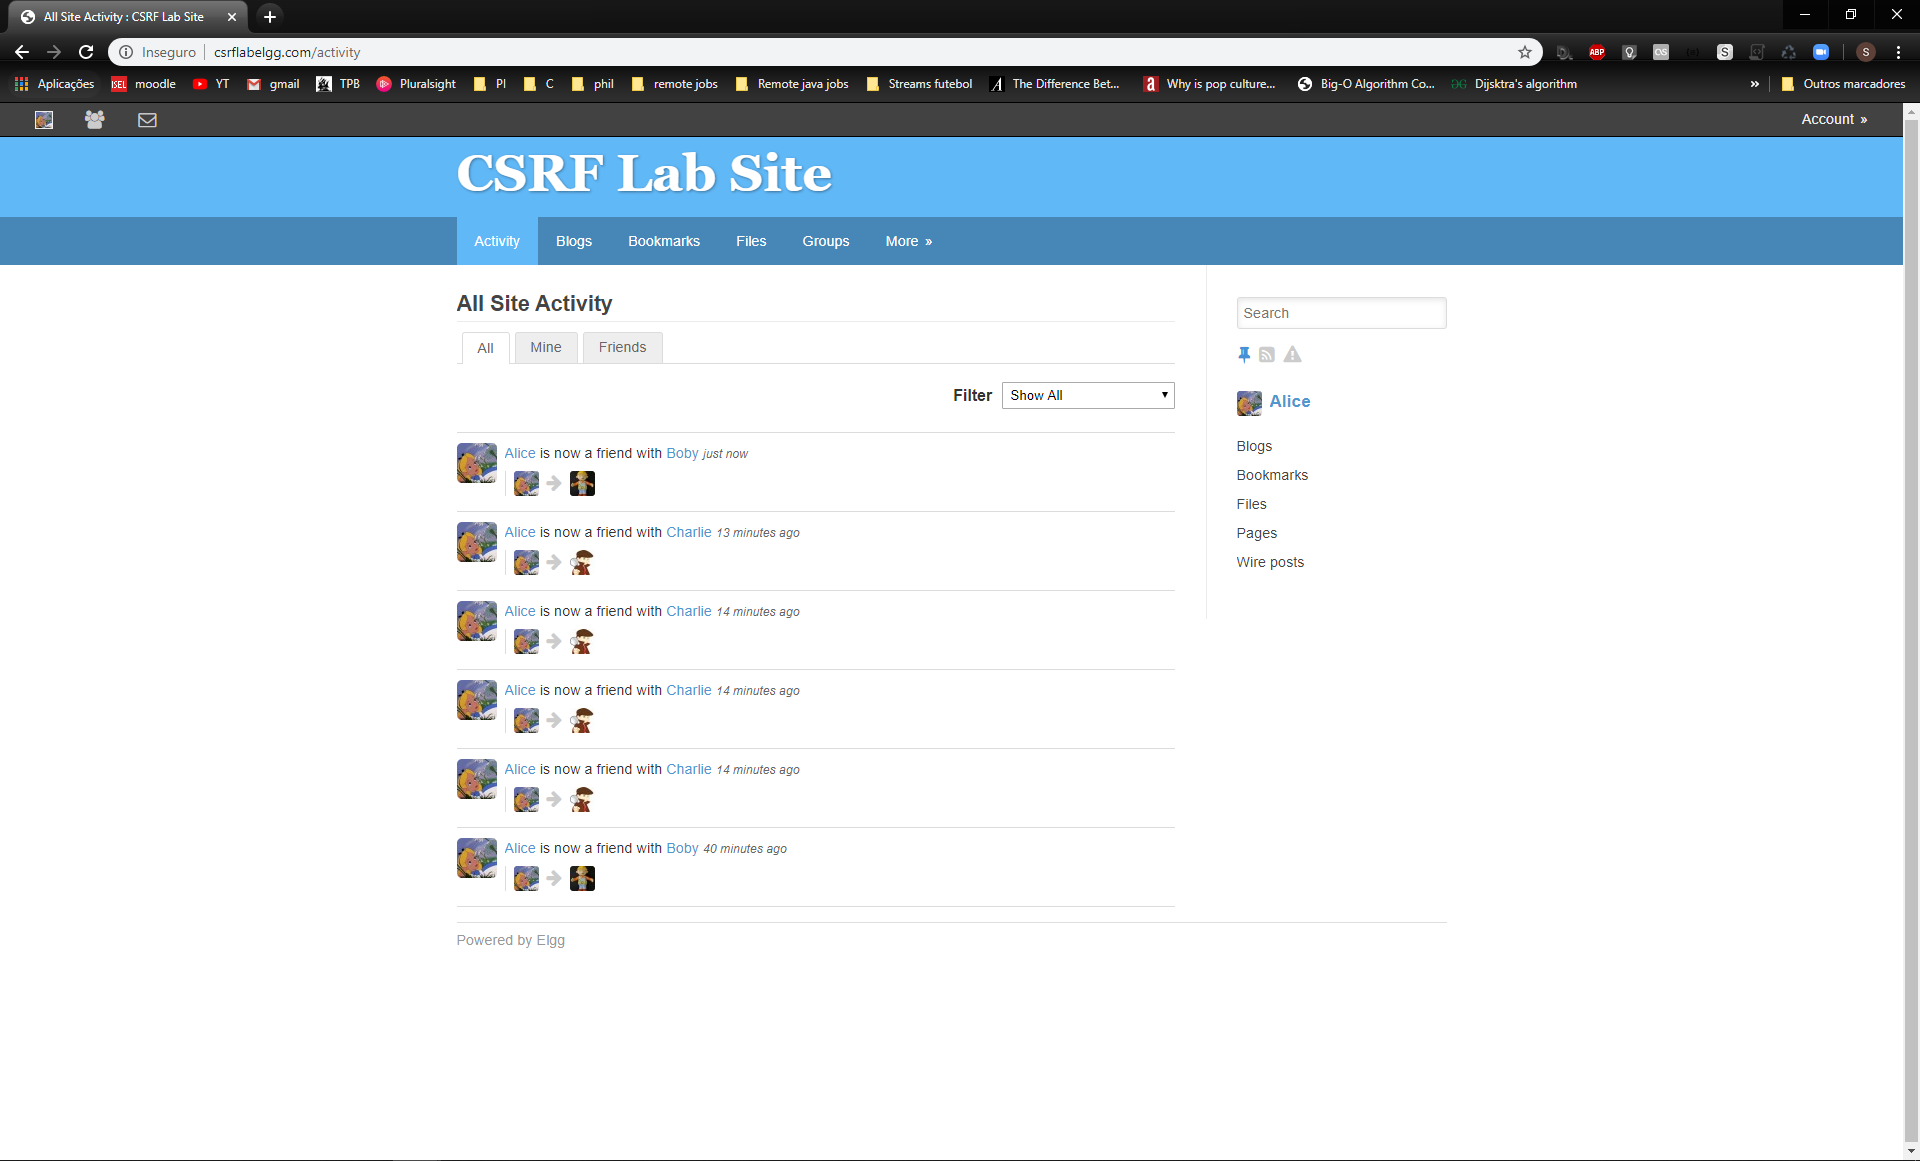
\includegraphics[width=\linewidth]{img/done}
	\caption{Como efeito do ataque, Alice é agora amiga de Boby}
	\label{fig:done}
\end{figure}




\end{document}
